\section{Exploration du modèle de Beremin}

Le modèle de Beremin suppose que dans tout volume élémentaire $V_0$, la taille $a$ des défauts susceptibles
de provoquer le clivage est régie par une densité de probabilité en loi puissance :
\begin{equation}
p(a) = \alpha a^{-\beta}
\end{equation}
avec $\alpha > 0$ et $\beta > 1$.

\begin{questions}
\question En considérant un critère de Griffith pour la propagation de micro-défauts, montrer que la probabilité de rupture sous une contrainte $\sigma$ donnée s'écrit en:
\begin{equation}
P(\sigma) \propto \sigma^m
\end{equation}
où $m$ s'exprime en fonction de $\beta$.

\begin{solution}
Pour que sous une contrainte $\sigma$, il y ait propagation instable d'une fissure à partir d'un défaut de taille $a$, il faut que le taux de restitution d'énergie dépasse une valeur critique. Cela se produit pour des défauts d'une taille supérieure à une valeur critique, $a_c$. Pour une fissure en forme de sou (\textit{penny-shape}), le facteur d'intensité de contrainte et le taux de restitution d'énergie s'écrivent :
$$ K_I = 2\sigma\sqrt{\dfrac{a}{\pi}}$$
$$ \mathcal{G} = \dfrac{(1-\nu^2)}{E}K_I^2 = \dfrac{4(1-\nu^2)}{\pi E}a \sigma^2$$
Le critère de Griffith s'écrit alors $\mathcal{G} \leq \mathcal{G}_c$.
Ainsi la taille critique $a_c$ correspondant à la propagation instable d'un défaut s'obtient par $\mathcal{G} =\mathcal{G}_c$ soit:
$$ a_c(\sigma) = \dfrac{\pi E \mathcal{G}_c}{4(1-\nu^2)\sigma^2} = \dfrac{\pi E \gamma_s}{2(1-\nu^2)\sigma^2} $$
en notant $\mathcal{G}_c = 2\gamma_s$.

La probabilité de rupture correspond alors à la probabilité, pour une contrainte $\sigma$ donnée, de trouver un défaut de taille supérieure ou égale à $a_c$, soit:
$$ P(\sigma) = \int_{a_c(\sigma)}^\infty p(a)da = \left[\dfrac{\alpha}{1-\beta}a^{1-\beta}\right]_{a_c(\sigma)}^\infty = \dfrac{\alpha}{\beta-1}a_c^{1-\beta} = \dfrac{\alpha}{\beta-1}\left(\dfrac{\pi E \gamma_s}{2(1-\nu^2)}\right)^{1-\beta} \sigma^{2\beta-2}$$
On a donc bien:
$$P(\sigma) \propto \sigma^m$$
en identifiant $m=2\beta-2 > 0$.
\end{solution}

\question En introduisant la contrainte de normalisation $\sigma_u$ de sorte que
\begin{equation}
P(\sigma) =  \left(\dfrac{\sigma}{\sigma_u}\right)^m,
\end{equation}
relier $\sigma_u$ aux paramètres mécaniques et aux paramètres de distribution des défauts $\alpha,\beta$.
\begin{solution}
En reprenant les expressions précédentes, on a:
$$ P(\sigma) = \dfrac{2\alpha}{m}\left(\dfrac{\pi E \gamma_s}{2(1-\nu^2)}\right)^{-m/2} \sigma^{m} = \dfrac{\sigma^m}{\dfrac{m}{2\alpha}\sqrt{\left(\dfrac{\pi E \gamma_s}{2(1-\nu^2)}\right)^m}}$$
On a alors:
$$\sigma_u = \left(\dfrac{m}{2\alpha}\right)^{1/m}\sqrt{\dfrac{\pi E \gamma_s}{2(1-\nu^2)}}.$$
\end{solution}

\subsection{Application à un acier bas carbone}
On considère dans la suite de cet exercice un acier à bas carbone s'appuyant sur les résultats de la thèse d’Astrid
Lambert-Perlade \cite{lambert2001rupture}. Ses propriétés en traction uniaxiale à
basse température (-170°C) sont les suivantes : limite d’élasticité 729 MPa, contrainte à rupture
978 MPa, allongement maximum réparti 11\%, allongement à rupture 25\%, réduction d’aire à rupture
78\%. 

\question Peut-on calibrer une loi de Weibull pour modéliser sa résistance à la rupture
fragile ?
\begin{solution}
La réduction d'aire à rupture est très élevée et suggère une rupture ductile, tout comme l'allongement à
rupture. Il est peu probable que ce type d'essai mette en évidence une rupture fragile. On ne peut donc
pas utiliser l'essai de traction uniaxiale pour cette caractérisation, sauf à abaisser encore la température
(et le résultat ne serait pas garanti).
\end{solution}

\subsection{Première estimation de la valeur du paramètre $m$}

Afin d’estimer le paramètre $m$ on utilise une comparaison entre le modèle de Beremin et le modèle de
\cite{curry1979effect}. Ce dernier fait appel à une modélisation du comportement en traction uniaxiale
via une loi puissance, $n$ étant l’exposant d’écrouissage. La valeur de $n$ est comprise entre 0.13 et 0.16
(selon la température) pour l’acier considéré. On pose ici $N = 1/n$.

Les relations entre la ténacité (en déformations planes) et la limite d’élasticité sont les suivantes, pour
chacun des modèles :
\begin{align*}
\text{Curry et Knott:}\quad & K_\text{Ic}\sigma_y^{\frac{N-1}{2}} = \text{constante}\\
\text{Beremin:}\quad & K_\text{Ic}\sigma_y^{\frac{m}{4}-1} = \text{constante}
\end{align*}

\question Utiliser ces deux expressions pour déduire un premier estimateur de $m$. Quelle est sa sensibilité
envers l’exposant d’écrouissage ?
\begin{solution}
Il vient $\frac{N-1}{2} = \frac{m}{4}-1$, d’où $m=2+2N=2+2/n$. Les valeurs numériques sont reportées dans le
tableau \ref{tab}. L’écart relatif entre les valeurs de $m$ est d’environ 20\% dans l’intervalle de détermination
utilisé.

\begin{R_table}
\begin{tabular}{|c|c|c|c|c|}
\hline 
$n$ & 0.13 & 0.14 & 0.15 & 0.16 \\ 
\hline 
Estimateur de $m$ & 17.38 & 16.29 & 15.33 & 14.50 \\ 
\hline 
\end{tabular}
\captionof{table}{Première estimation de $m$ via le modèle de \cite{curry1979effect}}\label{tab}
\end{R_table} 
\end{solution}
\end{questions}

\section{Application du modèle de Beremin à des essais de traction sur éprouvettes axisymétriques entaillées}

\subsection{Comportement macroscopique à rupture}

\begin{figure}
\begin{center}
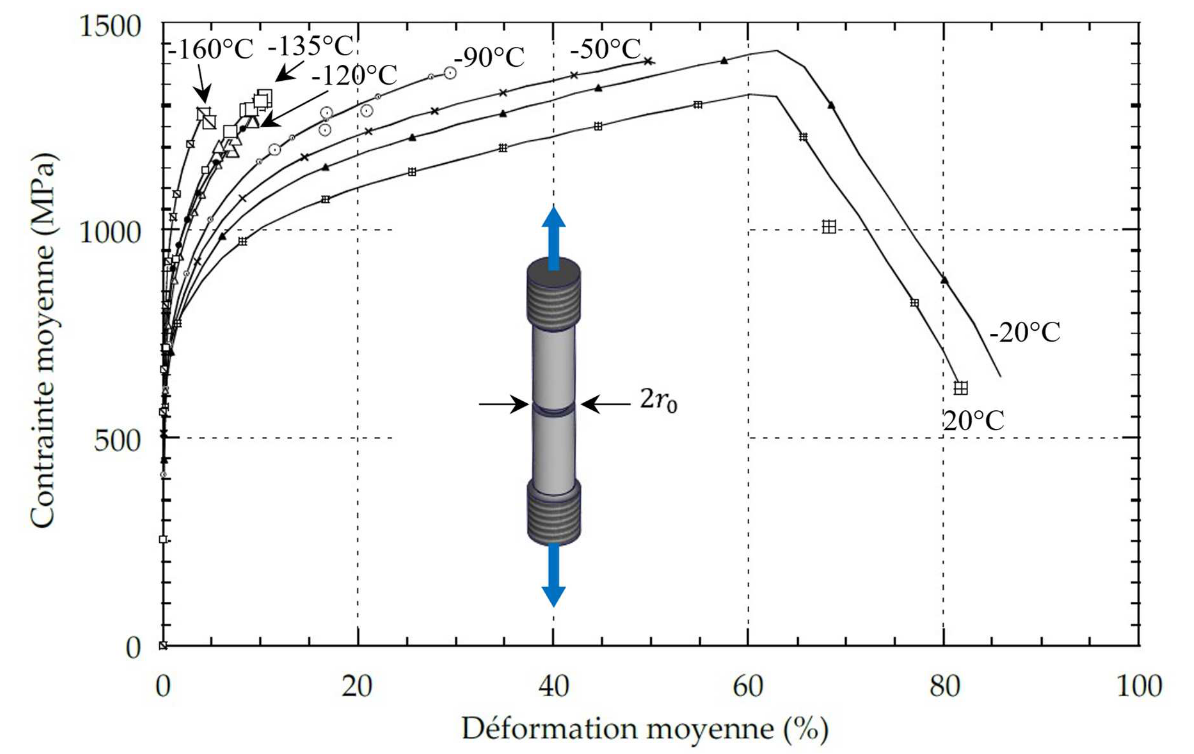
\includegraphics[width=0.8\textwidth]{courbes_traction_acier_bas_carbone}
\end{center}
\caption{Exemples de courbes de traction sur éprouvettes axisymétriques entaillées. Les
températures d’essai sont indiquées près des courbes correspondantes.}\label{fig:traction-acier}
\end{figure}

La Figure \ref{fig:traction-acier} montre quelques courbes d’essais de traction sur éprouvettes axisymétriques entaillées. La
contrainte moyenne (ou « contrainte nette ») est définie par le rapport entre l’effort de traction et l’aire
initiale de la section au droit du fond d’entaille. La déformation moyenne est définie de la manière
suivante : $\overline{\varepsilon} = 2\log(r/r_0)$, $r$ étant le rayon de l’éprouvette au droit du fond d’entaille, de valeur initiale $r_0$.

\begin{questions}
\question Qualifier le comportement macroscopique à rupture de ces éprouvettes, en fonction de la température.

\begin{solution}
A +20°C et -20°C, la courbe passe par un maximum puis l’effort chute, sans doute du fait d’une
réduction d’aire importante. Le comportement macroscopique est donc ductile.
A partir de -50°C et au-dessous, l’éprouvette casse avant que la charge ait atteint un maximum. Plus la
température est basse et plus la déformation moyenne à rupture est faible, passant de 50\% à -50°C à
moins de 10\% à -160°C. Le comportement devient plastique fragile, en particulier à partir de -120°C.
\end{solution}

\subsection{Détermination de la valeur de la contrainte à utiliser dans le modèle de Beremin}
On considère ici les essais réalisés à des températures inférieures ou égales à -90°C.

\question Déterminer l’intervalle des valeurs de contrainte nette à rupture. Peut-on utiliser ces valeurs pour caler les paramètres du modèle de Beremin ? Pourquoi ?
\begin{solution}
Les valeurs de la contrainte nette à rupture s’étendent d’environ 1250 MPa à environ 1350 MPa. Ce sont des valeurs moyennes de la contrainte axiale, qui est bien la contrainte principale maximale mais elle est hétérogène dans la section. L’amorçage du clivage a lieu dans une région de l’éprouvette où la contrainte est généralement différente de cette valeur moyenne. Il faut donc localiser le lieu de chaque amorçage et estimer la contrainte correspondante en utilisant un modèle de comportement mécanique, généralement via une simulation numérique.
\end{solution}

\subsection{Algorithme d’identification des paramètres du modèle de Beremin}

\question Quelles prédictions du modèle de Beremin utilise-t-on pour comparer avec les données
d’origine expérimentale ?
\begin{solution}
Pour comparer données expérimentales et prédictions du modèle de rupture, on utilise la
distribution de probabilité de la contrainte de Weibull à rupture. Cette courbe est donnée dans
le modèle de Beremin par $P_f(\sigma_W) = 1-\exp\left(-\left(\dfrac{\sigma_W}{\sigma_u}\right)^m\right)$ où la contrainte de Weibull est donnée par:
$$\sigma_W = \left(\int_{\text{PZ}} \sigma_1^m \dfrac{dV}{V_0} \right)^{1/m},$$
correspondant au moment d'ordre $m$ de la distribution de la contrainte principale majeure sur la zone plastique.
\end{solution}
\question Comment classer les essais sur éprouvettes axisymétriques entaillées de manière à tracer les
courbes en question ?
\begin{solution}
Selon la localisation du site d’amorçage, et en présence d’une déformation plastique importante avant rupture, la contrainte principale maximale peut être passée par un maximum avant le moment de la rupture. Quelle valeur faut-il alors prendre dans le calcul de $\sigma_W$ ? Pour s’affranchir de cette difficulté, on utilise une observable strictement croissante, la déformation à rupture. Aux très basses températures, lorsque le comportement est très fragile (comme ici à -90°C et en dessous), la contrainte principale maximale au site d’amorçage est également croissante au cours de l’essai et le problème ne se pose pas pour le calcul de $\sigma_W$.
\end{solution}

\question Proposer une méthode de détermination des paramètres du modèle de Beremin, en supposant
que l’analyse mécanique des essais a été effectuée au préalable par simulation numérique,
appuyée sur un modèle de comportement élasto-plastique adéquat.

\begin{solution}
Pour déterminer les paramètres de Beremin, il faut calculer une contrainte de Weibull à rupture pour chaque essai et comparer l’ensemble des valeurs $P_f(\sigma_W)$ avec les prédictions du modèle. On utilise donc un post-traitement des calculs en élasto-plasticité, pour chaque température d’essai mais aussi pour chaque essai individuel, du fait de la dispersion des valeurs à rupture. On calcule ensuite l’écart entre les données expérimentales et la prédiction, par exemple, par une méthode des moindres carrés, pour optimiser le couple $(m,\sigma_u)$.
\end{solution}

\question Justifier qu’une procédure itérative est indispensable.
\begin{solution}
La contrainte de Weibull, $\sigma_W$, est le moment d’ordre $m$ de la contrainte principale maximale sur l’ensemble de la zone plastique. Sa valeur dépend donc de $m$. Les données « expérimentales » dépendent ainsi des paramètres du modèle! Il faut donc répéter le calcul de $\sigma_W$ pour chaque éprouvette, pour chaque boucle d’optimisation du couple $(m,\sigma_u)$. La méthode est intrinsèquement itérative. On peut partir d’une valeur initiale de $m$ donnée, par exemple, par l’utilisation du modèle de Curry et Knott comme cela a été fait dans l’exercice précédent. 
\end{solution}

\subsection{Discussion des résultats de l’ajustement}
La mise en \oe{}uvre de cette méthode sur les 25 essais disponibles donne $m=20$ et $\sigma_u=\SI{2351}{MPa}$ pour
un volume $V_0$ de $(\SI{100}{\micro\meter})^3$. Le résultat est représenté sur la Figure \ref{fig:Beremin-results}.
\begin{figure}
\begin{center}
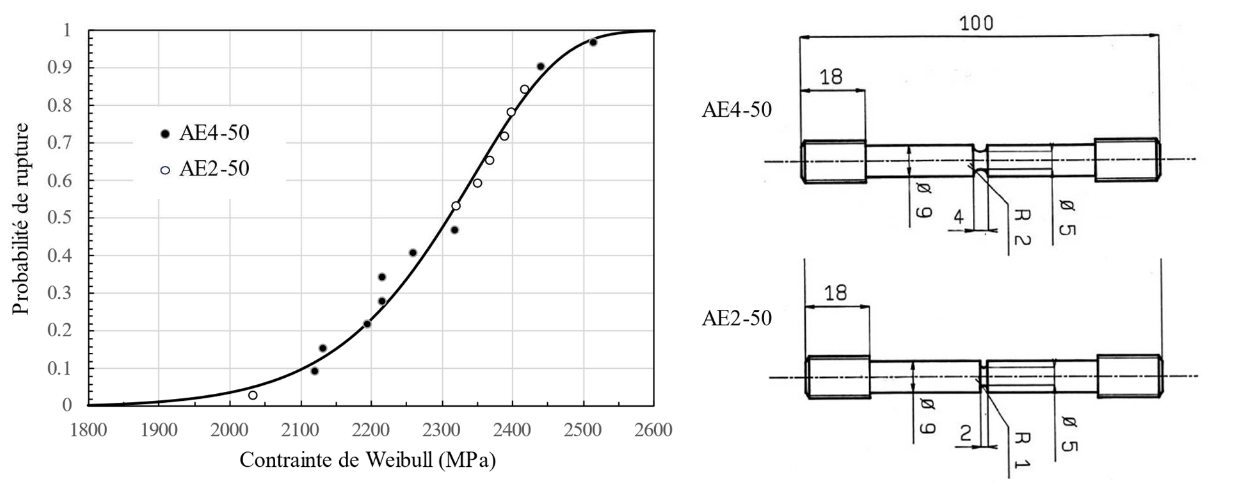
\includegraphics[width=\textwidth]{resutats_Beremin}
\end{center}
\caption{Ajustement des paramètres du modèle de Weibull sur les données d’essais de traction sur
éprouvettes axisymétriques entaillées. Les deux géométries sont représentées à côté du graphe, avec
les cotes en millimètres.}\label{fig:Beremin-results}
\end{figure}

\question Commenter la qualité de l’ajustement des paramètres du modèle.
\begin{solution}
L'ajustement de la courbe $P_f(\sigma_W)$ par le modèle de Beremin semble de très bonne qualité sur l’ensemble de la distribution.
\end{solution}

\question Commenter la valeur de $m$ par rapport aux premières estimations faites à partir du modèle de Curry et Knott.
\begin{solution}
La valeur de $m$ est légèrement plus haute que la valeur estimée via le modèle de Curry et
Knott. Pour information, l’intervalle de confiance, pour $m= 20$ et avec 25 essais sur éprouvettes axisymétriques entaillées, s’étend de 14.7 à 28.6.
\end{solution}

\question Commenter la valeur de $\sigma_u$ par rapport aux contraintes nettes à rupture déterminées à partir
des courbes de la Figure \ref{fig:traction-acier}.
\begin{solution}
La valeur de $\sigma_u$ ($\SI{2351}{MPa}$) est bien plus élevée que la contrainte nette ($1250$ à $\SI{1350}{MPa}$) :
du fait du moment d’ordre $m$ et de l'équivalence entre tous les volumes $V_0$ en termes de population de défauts, les valeurs élevées de contrainte locale sur sur-représentées dans le calcul de $\sigma_W$. On rappelle en outre que les valeurs de $m$ et de $V_0$ ne sont pas indépendantes, puisque la distribution de défauts est paramétrée pour une valeur donnée de $V_0$.
\end{solution}

\end{questions}

